\documentclass{beamer}
\mode<presentation>{
	\usetheme{Madrid}
	\usecolortheme{beaver}
}
\usepackage{graphicx}
\usepackage{listings}
\graphicspath{{./images}}
\usepackage[backend=bibtex, sorting=none]{biblatex}
\addbibresource{./bibliography/bib.bib}
\usepackage{polski}
\title[]{Implementacja systemu rekomendacji filmów opartego na grafowej bazie danych}
\institute[UMCS]
{
	Uniwersytet Marii Curie Skłodowskiej
	\medskip
}
\author{Sebastian Tyda}
\date{\today}

\begin{document}
	% 1
	\begin{frame}
		\titlepage
	\end{frame}
	% 2
	\begin{frame}
		\frametitle{Cel pracy}
		\section{Cel pracy}
		\begin{itemize}
			\item Przybliżenie systemów rekomendacji i algorytmów rankingowych
			\item Omówienie zagadnienia ontologii i grafowych baz danych
			\item Opracowanie architektury systemu
			\item Implementacja - opracowanie ontologii, utworzenie bazy, implementacja wybranego algorytmu rankingowego oraz opracowanie uproszczonej aplikacji
		\end{itemize}
	\end{frame}

	% 3
	\begin{frame}
		\frametitle{Istota pracy}
		\section{Istota pracy}
		\begin{itemize}
			\item Pokazanie netflixowi gdzie raki zimują
		\end{itemize}
	\end{frame}

	% 4
	\begin{frame}
		\frametitle{Systemy rekomendacji}
		\section{Systemy rekomendacji}
		\begin{itemize}
			\item Collaborative filtering
			\item Content/Knowledge-based Filtering
			\item Session-based
			\item Personalized Learning to Rank
			\item Context Aware Recommendation
			\item Other: Demographic, Social(Trust), Deep Learning
			\item Hybrid Systems
		\end{itemize}
	\end{frame}

	% 5
	\begin{frame}
		\frametitle{Algorytmy rankingowe}
		\section{Algorytmy rankingowe}
		\begin{itemize}
			\item Boolean Models
			\item Vector Space Model
			\item Probabilistic Model
			\item PageRank
			\item HITS Algorithm
			\item Okapi BM25
			\item Weighted AND
		\end{itemize}
	\end{frame}

	% 6
	\begin{frame}
		\frametitle{Ontologie}
		\section{Ontologie}
		Ontologia – formalna reprezentacja pewnej dziedziny wiedzy, na którą składa się zapis zbiorów pojęć i relacji między nimi.
		\newline
		\newline
		Języki zapisu ontologii:
		\begin{itemize}
			\item OWL (Web Ontology Language)
			\item RDF (Resource Description Framework)
			\item RDF Vocabulary Description Language (RDF Schema, RDFS)
		\end{itemize}
	\end{frame}

	% 7
	\begin{frame}
		\frametitle{Grafowe bazy danych}
		\section{Grafowe bazy danych}
		Grafowa baza danych – baza danych wykorzystująca struktury grafów z węzłami, krawędziami i własnościami do przedstawiania i przechowywania danych oraz do obsługi zapytań semantycznych.
		\begin{center}
			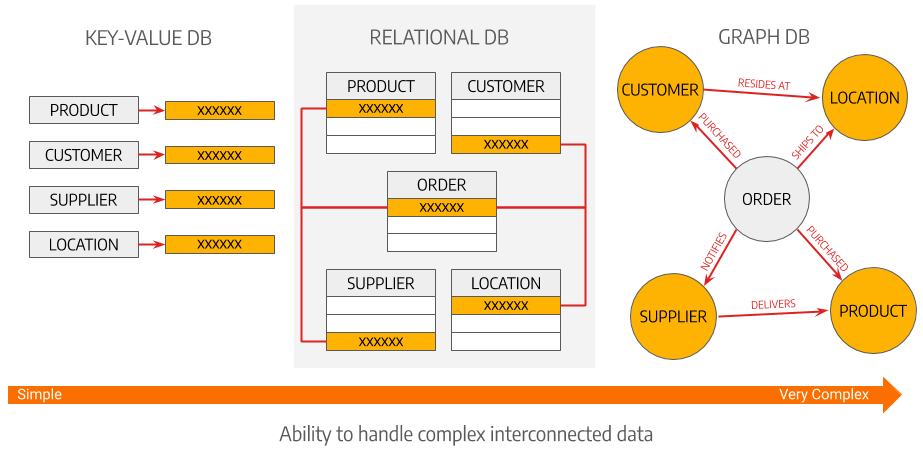
\includegraphics[scale=0.30]{graph}
		\end{center}
	\end{frame}

	% 8
	\begin{frame}
		\frametitle{Przykłady datasetów}
		\section{Przykłady datasetów}
		\begin{itemize}
			\item \href{https://www.dbpedia.org}{DBpedia}
			\item \url{https://www.kaggle.com/rounakbanik/the-movies-dataset} (metadane dla ponad 45,000 filmów, 26 milionów ocen od ponad 270 tysięcy użytkowników)
		\end{itemize}
	\end{frame}

	% 9
	\begin{frame}
		\frametitle{Biblioteki pythona}
		\section{Biblioteki pythona}
		\begin{itemize}
			\item RDFLib
			\item Owlready2
		\end{itemize}
	\end{frame}

	% 10
	\begin{frame}
		\frametitle{}
		\section{}
		\begin{center}
			\Huge Dziękuję za uwagę!
		\end{center}
	\end{frame}

\end{document}